\documentclass[tikz,border=10pt]{standalone}
\usepackage{lmodern}
\usepackage[T1]{fontenc}
\usepackage{tikz}
\usetikzlibrary{arrows.meta,positioning,calc}
% Shared color palette for figures (not compiled on its own)
\definecolor{ink}{HTML}{1C1917}
\definecolor{crimson}{HTML}{8A1F1B}
\definecolor{navy}{HTML}{243B55}
\definecolor{gold}{HTML}{B08D3E}
\definecolor{cream}{HTML}{F7F1E8}
\definecolor{sand}{HTML}{E8DCC8}
\definecolor{mist}{HTML}{D7E1EA}
\definecolor{mid}{HTML}{6B8AA3}
\definecolor{deep}{HTML}{3D1F1E}

\begin{document}
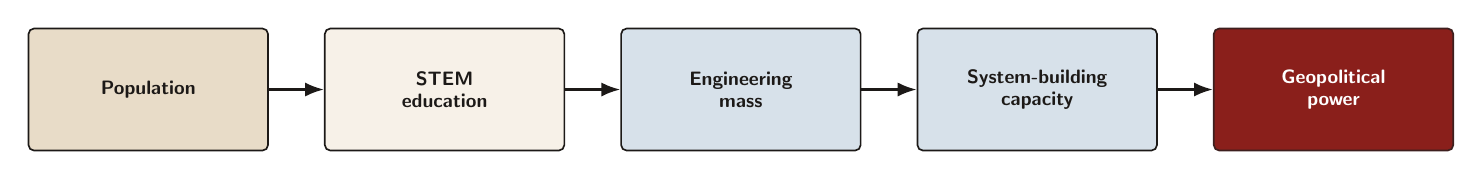
\begin{tikzpicture}[
  font=\sffamily,
  box/.style={draw=ink, line width=0.6pt, rounded corners=2pt,
    align=center, text=ink, fill=cream, inner sep=7pt, font=\sffamily\bfseries\scriptsize,
    text width=2.55cm, minimum height=1.55cm},
  arr/.style={-{Latex[length=2.4mm]}, ink, line width=0.9pt}
]
  \node[box, fill=sand] (a) {Population};
  \node[box, right=7mm of a] (b) {STEM\\education};
  \node[box, right=7mm of b, fill=mist] (c) {Engineering\\mass};
  \node[box, right=7mm of c, fill=mist] (d) {System-building\\capacity};
  \node[box, right=7mm of d, fill=crimson, text=white, draw=deep] (e) {Geopolitical\\power};
  \draw[arr] (a) -- (b);
  \draw[arr] (b) -- (c);
  \draw[arr] (c) -- (d);
  \draw[arr] (d) -- (e);
\end{tikzpicture}
\end{document}
